\section{Cubic Basis-Functions} \label{cha:Cubic_Basis_Function}
Cubic polynomial basis functions are widely used in FEM, including in one-dimensional problems.
There are several reasons for this popularity:
\begin{enumerate}
	\item Cubic basis functions support \glsentryname{order1Cont}, producing a smoother solution than the linear choice.

	\item They generally provide a more accurate solution and a higher convergence rate than the linear case.

	\item The additional cost of using cubic rather than linear basis functions is modest, especially in one dimension.
\end{enumerate}
%
In the linear case, one basis function was associated with each node, giving $N+1$ functions and two shape functions per element.

In the cubic case, on the other hand, we need $4$ \glspl{shapeFunction} over each \gls{element}, or totally $2N + 2$ \glspl{basisFunction}.
Each cubic \gls{shapeFunction} has 4 parameters and thus must have $4$ conditions to be fully specified. The first $2$ conditions
concern function values at the \glspl{nodePoint}, while the last $2$ give values of first derivatives at the same node points. \\

The first \gls{shapeFunction} $\psi_1$, guarantees function values $1$ and $0$ on the left and right element boundaries, as well as a
vanishing derivative at both ends
\begin{subequations}	\label{eqn:Cond_On_Cubic_Psi_1_Local}
	{\allowdisplaybreaks
		\begin{align}
			\psi_{1} \left( 0\right) &= 1,	\\
			\psi_{1} \left( 1 \right) &= 0,	\\
			\psi_{1,  x}\left( 0 \right) &= 0,	\\
			\psi_{1,  x}\left( 1 \right) &= 0.
		\end{align}
	}% end of \allowdisplaybreaks
\end{subequations}
The second \gls{shapeFunction} has a value of unity at the right boundary, otherwise function and derivative values of zero at the boundaries.
In the same manner the third and fourth \glspl{shapeFunction} have their unity values for the derivative at the left and right boundaries.	\\

A general cubic polynomial and its derivative may be written as
\begin{subequations}
	\begin{align}
		\psi _{i}\left( x \right) &= c_{0} + c_{1} x + c_{2}x^{2} + c_{3}x^{3},	\label{eqn:General_Cubic_Func}	\\
		\psi _{i}^{\prime} \left( x \right) &= c_{1} + 2c_{2}x + 3c_{3}x^{2}.	\label{eqn:General_Cubic_Der}
	\end{align}
\end{subequations}
%
For each \gls{shapeFunction} coefficients $c_1, \dots, c_4$ may be found by applying conditions above to
\cref{eqn:General_Cubic_Func,eqn:General_Cubic_Der}. Here are the results
\begin{subequations}	\label{eqn:Cubic_Psi_Local}
	\begin{align}
		\psi _{1}\left( x \right) &= 1 - 3 x^{2} + 2x^{3},	\\
		\psi _{2}\left( x \right) &= 3 x^{2} - 2 x^{3},	\\
		\psi _{3}\left( x \right) &= x - 2 x^{2} + x^{3},	\\
		\psi _{4}\left( x \right) &= -x^{2} + x^{3}.
	\end{align}
\end{subequations}
%
Cubic \glspl{shapeFunction} and \gls{piecewiseCubic}
polynomials over the whole domain are depicted in \cref{fig:Cubic_Shape_Functions,fig:Cubic_Basis_Functions}, respectively. Observe
from the latter that the first $N+1$ functions control the solution value at \glspl{nodePoint}, while the last $N+1$ functions
take care of first derivatives at \glspl{nodePoint}. \\	\\
Thus using \cref{eqn:Truncated_FEM_Solution} with $M = 2N + 2$, the solution value at \glspl{nodePoint} may be written as
\begin{subequations}
	\begin{align}
		% Function u(x)
		\gls{u} &= \sum_{i = 1}^{2N + 2} \glsentryname{ai} \gls{phii},	\notag \\
		% Function value at x = x_j
		\glsentryname{uAtXj} &= \sum_{i = 1}^{2N + 2} \glsentryname{ai} \gls{phii} \bigg \vert_{x = x_j} = a_j,	\label{eqn:Cubic_Solution_At_X_i}
	\end{align}
	In the same manner we apply \cref{eqn:u_Prime} with $M = 2N + 2$ to find the first derivative values at the \glspl{nodePoint}, i.e.,
	\begin{equation}
		% First derivate at x_j,
		\glsentryname{uPrimeAtXj} = \sum_{i = 1}^{2N + 2} a_i \glsentryname{phiiPrime} \bigg \vert_{x = x_j}
		= a_{j + N + 1}.	\label{eqn:Cubic_Solution_Derivative_At_X_i}
	\end{equation}
\end{subequations}
%
Thus the cubic choice results in $M = 2N + 2$ \glspl{dof}. \Glspl{shapeFunction} and their derivatives, in both the linear and
cubic case are implemented in \cref{lst:Def_FEM_Func}.
\begin{figure}
	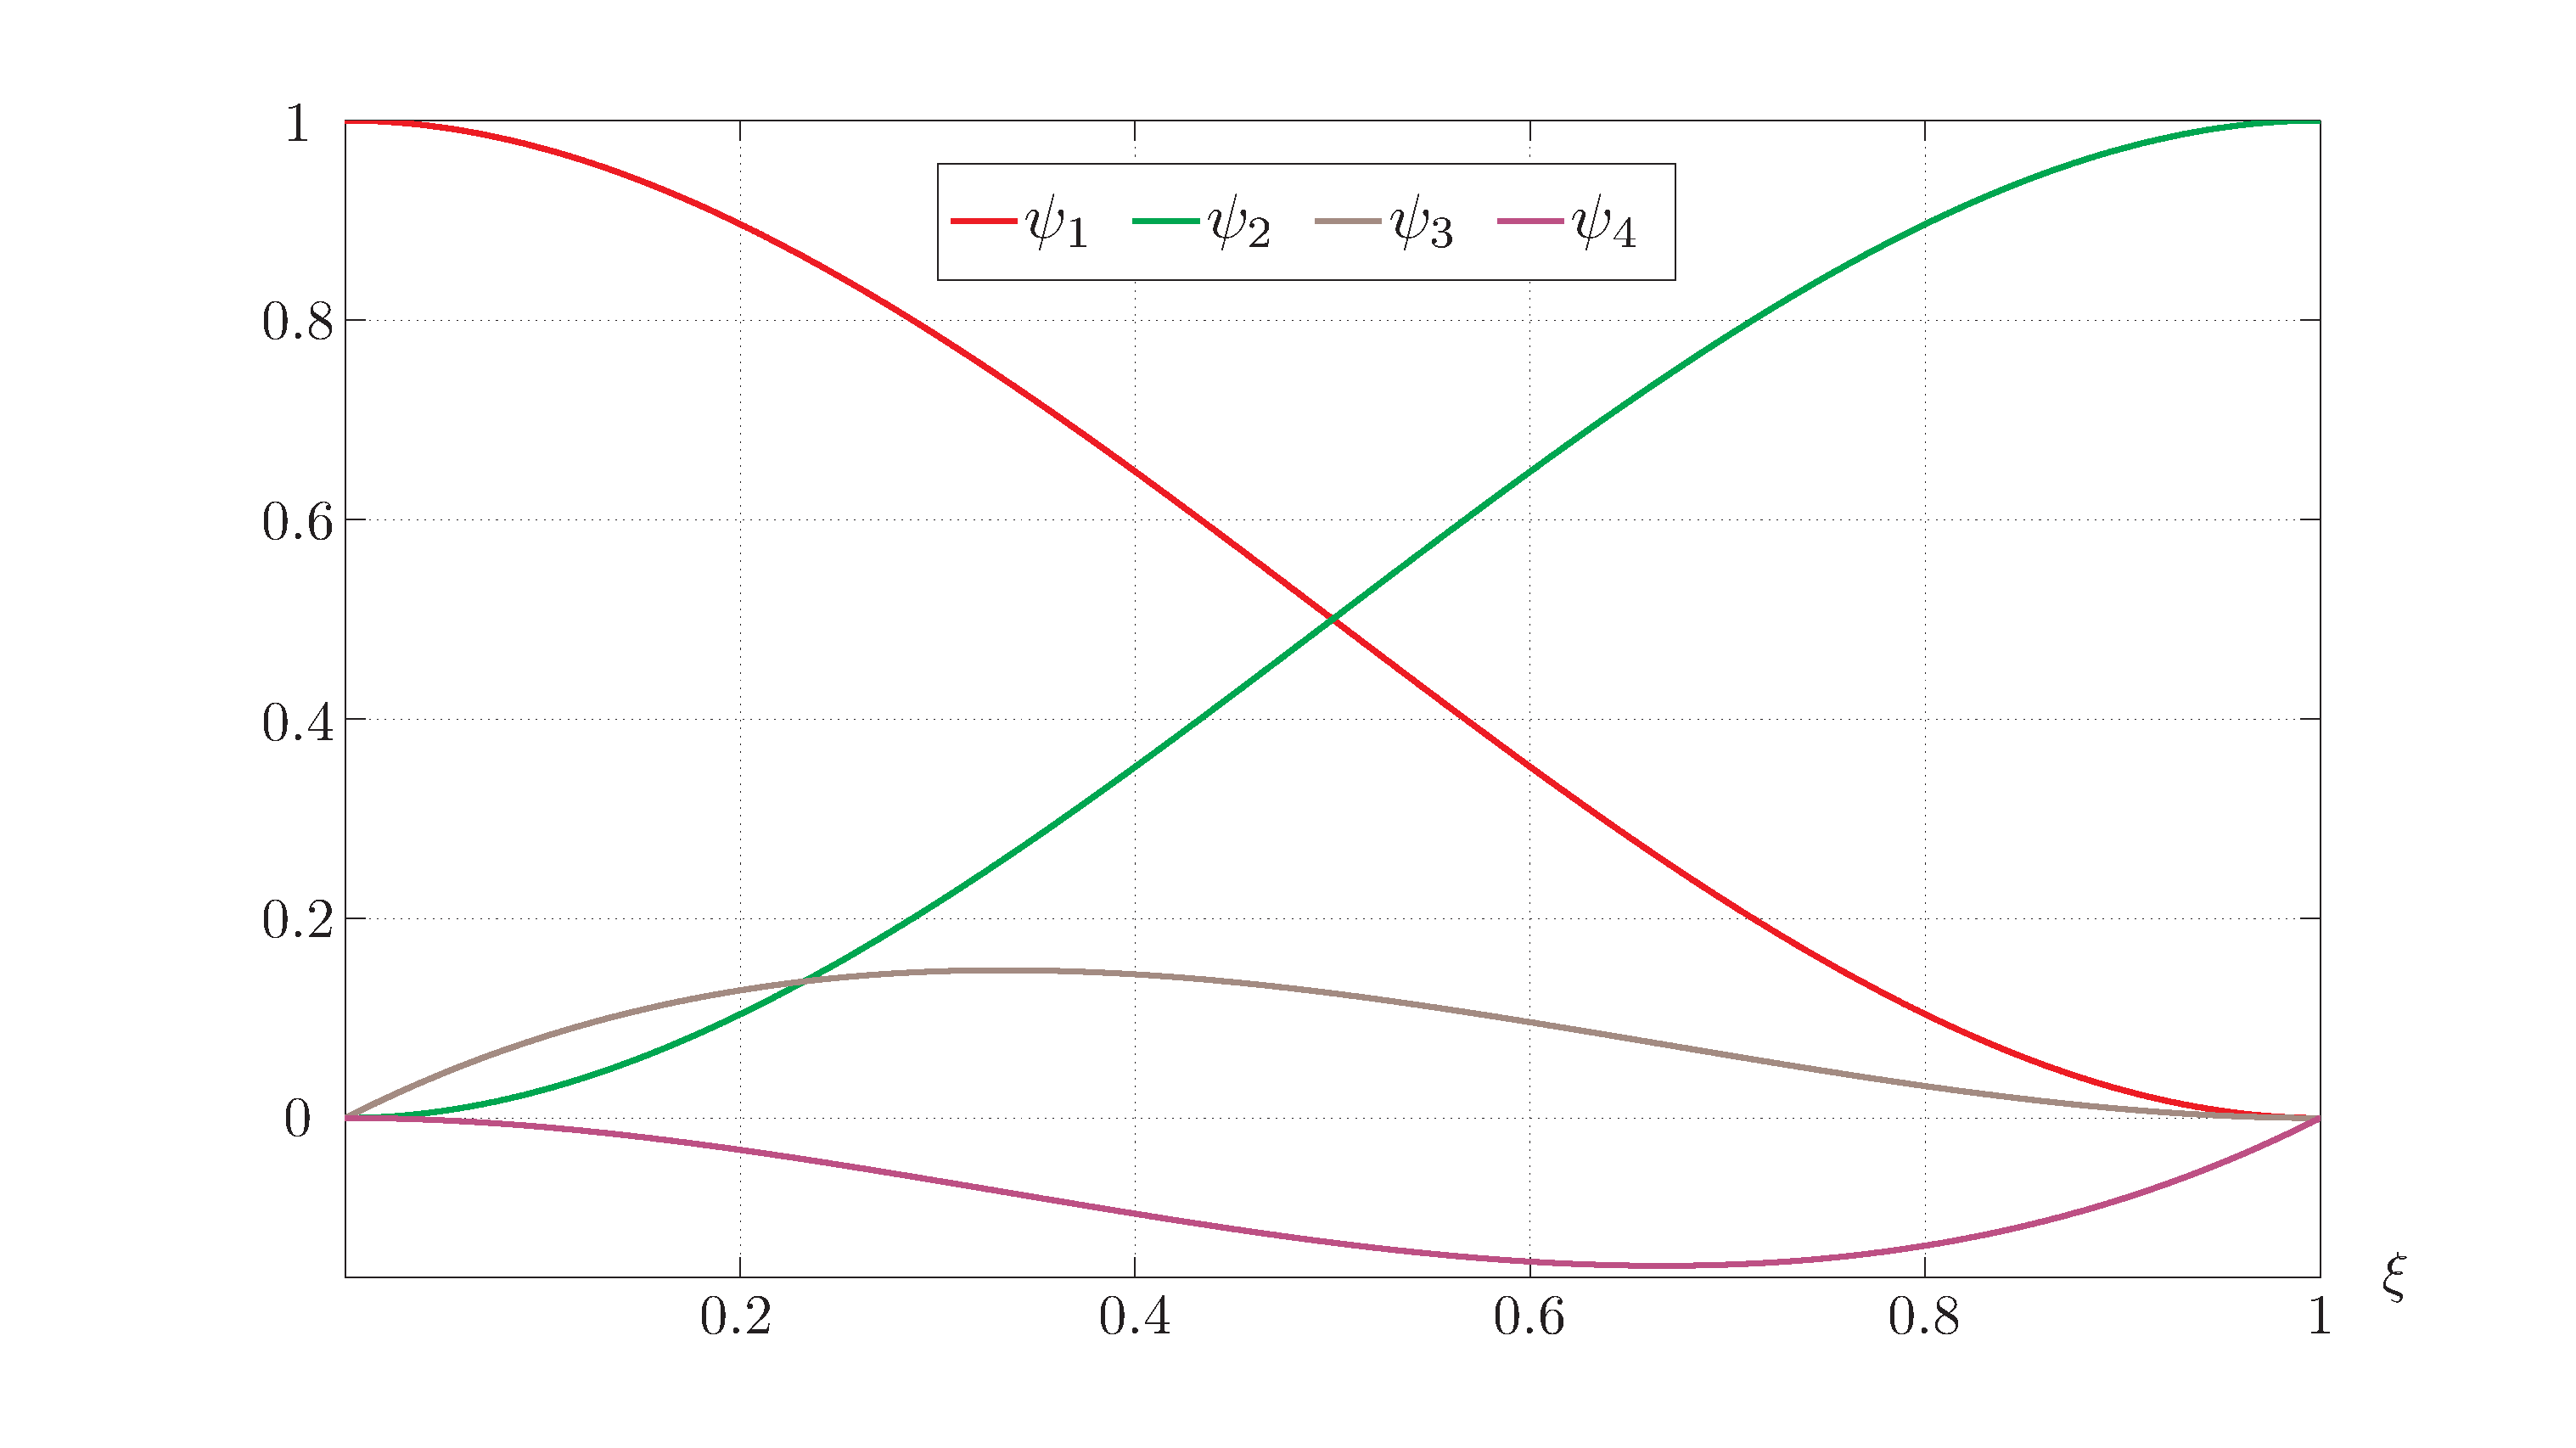
\includegraphics[width = \textwidth]{../figures/cubic-shape-functions}
	\caption[Choice of Cubic Polynomials for Shape-Functions]
		{Choice of Cubic Polynomials for Shape-Functions}
	\label{fig:Cubic_Shape_Functions}
\end{figure}
\begin{figure}
	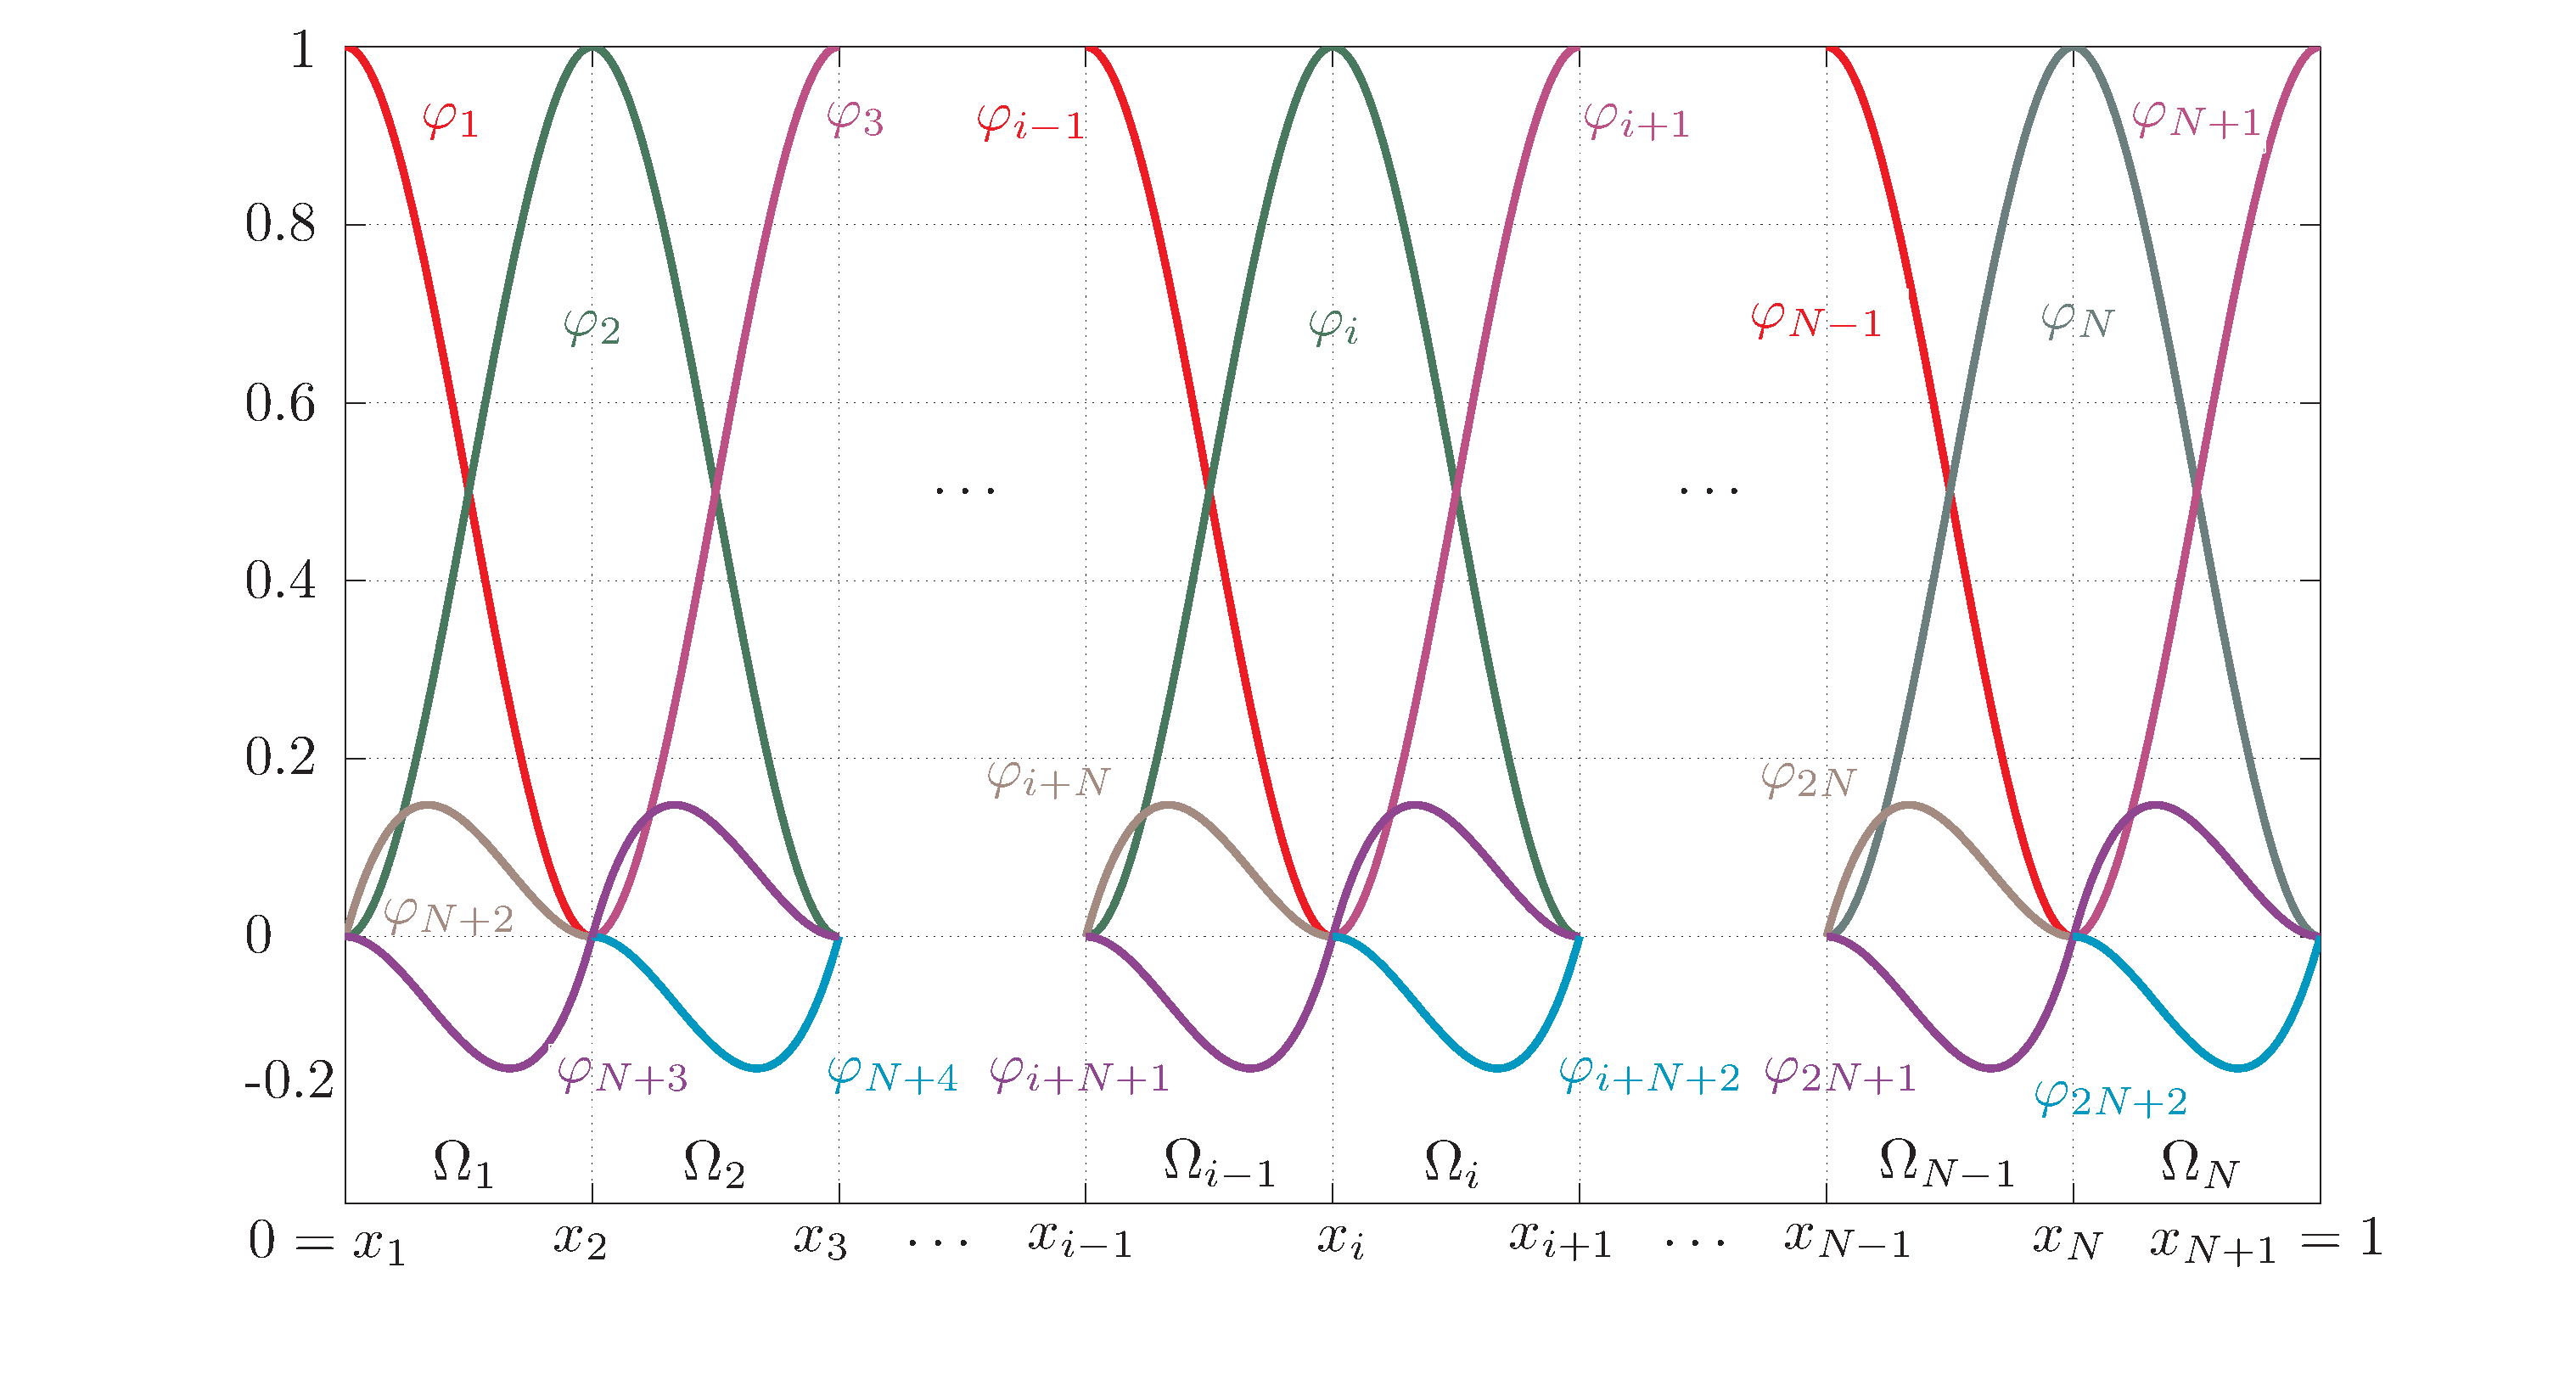
\includegraphics[width = \textwidth]{../figures/cubic-basis-functions}
	\caption[Choice of Cubic Polynomials for Basis-Functions]
		{Choice of cubic polynomials for Basis-Functions gives a solution which is $\mathcal{O} \left( 1 \right)$-continuous.}
	\label{fig:Cubic_Basis_Functions}
\end{figure}
%
\subsection[Element Matrix and Element Load]{\Gls{elementMatrix} and \Gls{elementLoad}} \label{cha:Element_Matrix_Load_Cubic}
Above we saw how we could calculate the global \gls{stiffnessMatrix} and \gls{loadVector} by summing element contributions,
see under \cref{cha:Element_Matrix_Linear,cha:Element_Load_Linear,cha:Assembly_Process_Linear}. Note that we defined
two \glspl{shapeFunction} over a typical \gls{element} in the linear case. The \gls{elementMatrix} and \gls{loadVector} for
\gls{linearFEMSol} are then \gls{Ke} $\in$ \glsentryname{R22} and \gls{be} $\in$ \glsentryname{R21}, respectively. In the cubic
case, on the other hand, there are $4$ nonzero \glspl{shapeFunction} over each \gls{element}. Thus
\begin{subequations}
	\begin{alignat}{2}
		\glsentryname{Kmne} &= \frac{1}{h} \int_{0}^{1} q \Bigl[ \left( e - 1 + \xi \right) h \Bigr] \frac{ d \psi_m }{ d \xi }
			\frac{ d \psi_n }{ d \xi } \dd \xi,	\quad& m, n = 1, \dots, 4,	\label{eqn:Cubic_Element_Stiffness_Entries}	\\
			b_{m}^{e} &= h \int_{ 0 }^{ 1 } f \biggl[ h \left( e - 1 + \xi \right) \biggr] \psi_m \left( \xi \right) \dd \xi,
				\quad& m = 1, \dots, 4.	\label{eqn:Cubic_Element_Load_Entries}
	\end{alignat}
\end{subequations}	\text{}
\Cref{lst:Elem_Cont} shows MATLAB code for implementation of element contributions in both linear and cubic case.
%
\subsection{Assembly Process} \label{cha:Assembly_Process_Cubic}
Again, denote by \gls{K} and \gls{b} the global \gls{stiffnessMatrix} and \gls{loadVector}. Also let \gls{KGlobalE} and
\gls{bGlobalE} describe status of \gls{K} and \gls{b} after addition of element and load contributions from elements
$1,2, \ldots, e$. Then assembly process with cubic basis functions are visualized in \crefrange{fig:K_1_Cubic}{fig:K_4_Cubic} and \cref{fig:b_1_To_b_4_Cubic}. MATLAB code in \cref{lst:Setup_Eq_Sys} implements this process in both linear and cubic case.

% ------------------ Insert Visualization of Cubic Assembly Process ------------------
% Cubic K^{1}
\begin{sidewaysfigure}[H]
	\centering
	\begin{equation*}
		\mathbf{K}^{\left( 1 \right)} =
		\begin{bmatrix}
			k_{11}^{1} & k_{12}^{1} & 0 & 0 & 0 & k_{13}^{1} & k_{14}^{1} & 0 & 0 & 0 \\ \\
			k_{21}^{1} & k_{22}^{1} & 0 & 0 & 0 & k_{23}^{1} & k_{24}^{1} & 0 & 0 & 0 \\ \\
			0 & 0 & 0 & 0 & 0 & 0 & 0 & 0 & 0 & 0 \\ \\
			0 & 0 & 0 & 0 & 0 & 0 & 0 & 0 & 0 & 0 \\ \\
			0 & 0 & 0 & 0 & 0 & 0 & 0 & 0 & 0 & 0 \\ \\
			k_{31}^{1} & k_{32}^{1} & 0 & 0 & 0 & k_{33}^{1} & k_{34}^{1} & 0 & 0 & 0 \\ \\
			k_{41}^{1} & k_{42}^{1} & 0 & 0 & 0 & k_{43}^{1} & k_{44}^{1} & 0 & 0 & 0 \\ \\
			0 & 0 & 0 & 0 & 0 & 0 & 0 & 0 & 0 & 0 \\ \\
			0 & 0 & 0 & 0 & 0 & 0 & 0 & 0 & 0 & 0 \\ \\
			0 & 0 & 0 & 0 & 0 & 0 & 0 & 0 & 0 & 0
			\end{bmatrix}
	\end{equation*}
	\caption{Stiffness Assembly with Cubic Basis-Functions, $\mathbf{K}^{\left( 1 \right)}$}
	\label{fig:K_1_Cubic}	
\end{sidewaysfigure}
%
% Cubic K^{2}
\begin{sidewaysfigure}[H]
	\centering
	\begin{equation*}
		\mathbf{K}^{\left( 2 \right)} =
		\begin{bmatrix}
			% 1. row
			k_{11}^{1} & k_{12}^{1} & 0 & 0	& 0 & k_{13}^{1} & k_{14}^{1} & 0 & 0 & 0 \\ \\
			% 2. row
			k_{21}^{1}&k_{22}^{1}+k_{11}^{2}&k_{12}^{2}&0 & 0 & k_{23}^{1} & k_{24}^{1}+k_{13}^{2} & k_{14}^{2} & 0 & 0 \\ \\
			% 3. row
			0 & k_{21}^{2} & k_{22}^{2} & 0 & 0 & 0 & k_{23}^{2} & k_{24}^{2} & 0 & 0 \\ \\
			% 4. row
			0 & 0 & 0 & 0 & 0 & 0 & 0 & 0 & 0 & 0 \\ \\
			% 5. row
			0 & 0 & 0 & 0 & 0 & 0 & 0 & 0 & 0 & 0 \\ \\
			% 6. row
			k_{31}^{1} & k_{32}^{1} & 0 & 0 & 0 & k_{33}^{1} & k_{34}^{1} & 0 & 0 & 0 \\ \\
			% 7. row
			k_{41}^{1}&k_{42}^{1}+k_{31}^{2}&k_{32}^{2}&0& 0 & k_{43}^{1} & k_{44}^{1}+k_{33}^{2} & k_{34}^{2} & 0 & 0 \\ \\
			% 8. row
			0 & k_{41}^{2} & k_{42}^{2} & 0 & 0	& k_{43}^{2} & k_{44}^{2} & 0 & 0 & 0 \\ \\
			% 9. row
			0 & 0 & 0 & 0 & 0 & 0 & 0 & 0 & 0 & 0 \\ \\
			% 10. row
			0 & 0 & 0 & 0 & 0 & 0 & 0 & 0 & 0 & 0
		\end{bmatrix}
	\end{equation*}
	\caption{Stiffness Assembly with Cubic Basis-Functions, $\mathbf{K}^{\left( 2 \right)}$}
	\label{fig:K_2_Cubic}
\end{sidewaysfigure}
%
% Cubic K^{3}
\begin{sidewaysfigure}[H]
	\centering
	\begin{equation*}
		\mathbf{K}^{\left( 3 \right)} =
		\begin{bmatrix}
			% 1. row
			k_{11}^{1} & k_{12}^{1} & 0 & 0 & 0 & k_{13}^{1} & k_{14}^{1} & 0 & 0 & 0 \\ \\
			% 2. row
			k_{21}^{1} & k_{22}^{1}+k_{11}^{2} & k_{12}^{2} & 0 & 0 & k_{23}^{1} & k_{24}^{1}+k_{13}^{2} & k_{14}^{2} & 0 & 0 \\ \\
			% 3. row
			0 & k_{21}^{2} & k_{22}^{2}+k_{11}^{3} & k_{12}^{3} & 0 & 0 & k_{23}^{2} & k_{24}^{2}+k_{13}^{3} & k_{14}^{3} & 0 \\ \\
			% 4. row
			0 & 0 & k_{21}^{3} & k_{22}^{3} & 0 & 0 & 0 & k_{23}^{3} & k_{24}^{3} & 0 \\ \\
			% 5. row
			0 & 0 & 0 & 0 & 0 & 0 & 0 & 0 & 0 & 0 \\ \\
			% 6. row
			k_{31}^{1} & k_{32}^{1} & 0 & 0 & 0 & k_{33}^{1} & k_{34}^{1} & 0 & 0 & 0 \\ \\
			% 7. row
			k_{41}^{1} & k_{42}^{1}+k_{31}^{2} & k_{32}^{2} & 0 & 0 & k_{43}^{1} & k_{44}^{1}+k_{33}^{2} & k_{34}^{2} & 0 & 0 \\ \\
			% 8. row
			0 & k_{41}^{2} & k_{42}^{2}+k_{31}^{3} & k_{32}^{3} & 0 & 0 & k_{43}^{2} & k_{44}^{2}+k_{33}^{3} & k_{34}^{3} & 0 \\ \\
			% 9. row
			0 & 0 & k_{41}^{3} & k_{42}^{3} & 0 & 0 & 0 & k_{43}^{3} & k_{44}^{3} & 0 \\ \\
			% 10. row
			0 & 0 & 0 & 0 & 0 & 0 & 0 & 0 & 0 & 0
		\end{bmatrix}
	\end{equation*}
	\caption{Stiffness Assembly with Cubic Basis-Functions, $\mathbf{K}^{\left( 3 \right)}$}
	\label{fig:K_3_Cubic}
\end{sidewaysfigure}
%
% Cubic K^{4}
\begin{sidewaysfigure}[H]
	\centering
	\begin{equation*}
		\mathbf{K}^{\left( 4 \right)} =
		\begin{bmatrix}
			% 1. row 
			k_{11}^{1} & k_{12}^{1}	& 0	& 0 & 0 & k_{13}^{1} & k_{14}^{1} & 0 & 0 & 0 \\ \\
			% 2. row
			k_{21}^{1}&k_{22}^{1}+k_{11}^{2} & k_{12}^{2} & 0 & 0 & k_{23}^{1} & k_{24}^{1}+k_{13}^{2} & k_{14}^{2} & 0 & 0 \\ \\
			% 3. row
			0&k_{21}^{2} & k_{22}^{2}+k_{11}^{3} & k_{12}^{3} & 0 & 0 & k_{23}^{2} & k_{24}^{2}+k_{13}^{3} & k_{14}^{3} & 0 \\ \\
			% 4. row
			0 & 0 & k_{21}^{3} & k_{22}^{3}+k_{11}^{4} & k_{12}^{4} & 0 & 0 & k_{23}^{3} & k_{24}^{3}+k_{13}^{4} & k_{14}^{4} \\ \\
			% 5. row
			0 & 0 & 0 & k_{21}^{4} & k_{22}^{4} & 0 & 0 & 0 & k_{23}^{4} & k_{24}^{4} \\ \\
			% 6. row
			k_{31}^{1} & k_{32}^{1} & 0 & 0 & 0 & k_{33}^{1} & k_{34}^{1} & 0 & 0 & 0 \\ \\
			% 7. row
			k_{41}^{1}&k_{42}^{1}+k_{31}^{2} & k_{32}^{2} & 0 & 0 & k_{43}^{1} & k_{44}^{1}+k_{33}^{2} & k_{34}^{2} & 0 & 0 \\ \\
			% 8. row
			0&k_{41}^{2} & k_{42}^{2}+k_{31}^{3} & k_{32}^{3} & 0 & 0 & k_{43}^{2} & k_{44}^{2}+k_{33}^{3} & k_{34}^{3} & 0 \\ \\
			% 9. row
			0 & 0 & k_{41}^{3} & k_{42}^{3} + k_{31}^{4} & 0 & 0 & 0 & k_{43}^{3} & k_{44}^{3} + k_{33}^{4} & k_{34}^{4} \\ \\
			% 10. row
			0 & 0 & 0 & k_{41}^{4} & k_{42}^{4} & 0 & 0 & 0 & k_{43}^{4} & k_{44}^{4}
		\end{bmatrix}
	\end{equation*}
	\caption{Stiffness Assembly with Cubic Basis-Functions, $\mathbf{K}^{\left(4\right)}$ }	
	\label{fig:K_4_Cubic}
\end{sidewaysfigure}
%
% Insert Cubic Load Assemby figure here
\begin{figure}[H]
	\centering
	\begin{equation*}
	\begin{aligned}
	% b_{1}
	\mathbf{b}^{\left( 1 \right)} &=
	\begin{bmatrix}
	b_{1}^{1} & b_{2}^{1} & 0 & 0 & 0 & b_{3}^{1} & b_{4}^{1} & 0 & 0 & 0
	\end{bmatrix}^{T},	\\
	% b_{2}
	\mathbf{b}^{\left( 2 \right)} &=
	\begin{bmatrix}
	b_{1}^{1} & b_{2}^{1} + b_{1}^{2} & b_{2}^{2} & 0 & 0 & b_{3}^{1} & b_{4}^{1} + b_{3}^{2} & b_{4}^{2} & 0 & 0
	\end{bmatrix}^{T},	\\
	% b_{3}
	\mathbf{b}^{\left( 3 \right)} &=
	\begin{bmatrix}
	b_{1}^{1} & b_{2}^{1} + b_{1}^{2} & b_{2}^{2} + b_{1}^{3} & b_{2}^{3} & 0 & b_{3}^{1} & b_{4}^{1} + b_{3}^{2} &
	b_{4}^{2} + b_{3}^{3} & b_{4}^{3} & 0
	\end{bmatrix}^T,	\\
	% b_{4}
	\mathbf{b}^{\left( 4 \right)} &=
	\begin{bmatrix}
	b_{1}^{1} & b_{2}^{1} + b_{1}^{2} & b_{2}^{2} + b_{1}^{3} & b_{2}^{3} + b_{1}^{4} & b_{2}^{4} & b_{3}^{1} &
	b_{4}^{1} + b_{3}^{2} & b_{4}^{2} + b_{3}^{3} & b_{4}^{3} + b_{3}^{4} & b_{4}^{4}
	\end{bmatrix}^{T}.
	\end{aligned}
	\end{equation*}
	\caption{Load Assembly with Cubic Basis-Functions, $\mathbf{b}^{\left(1\right)}, \dots, \mathbf{b}^{\left(4\right)}$}
	\label{fig:b_1_To_b_4_Cubic}
\end{figure}
%
%
Another way of explaining the assembly process follows:
\begin{enumerate}
	\item For each element $e$ calculate \gls{Ke} and \gls{be} from
	\cref{eqn:Cubic_Element_Stiffness_Entries,eqn:Cubic_Element_Load_Entries}.

	\item \Gls{elementMatrix} \gls{Ke} $\in$ \glsentryname{R44} may then be divided into $4$ sub-matrices all of them in \glsentryname{R22} i.e., upper/lower left and right. Add these sub-matrices to the global \gls{stiffnessMatrix} entries
	starting at entries $K_{e, e}$, $K_{e + N + 1, e}$, $K_{e, e + N + 1}$ and $K_{e + N + 1,e + N + 1}$, respectively.

	\item \Gls{elementLoad} \gls{be} $\in$ \glsentryname{R41}, on the other hand, is divided to two sub vectors of size
	$2\times 1$ each, i.e., upper and lower. These sub vectors are then added to the global \gls{loadVector} starting at entries
	$b_{e}$ and $b_{e + N + 1}$, respectively.
\end{enumerate}
%
\subsection[Implementation of Boundary Conditions]{Implementation of \glspl{boundaryCondition}}
The essential condition $u(0)=\delta$ is imposed directly on the left endpoint value degree of freedom. The natural condition in \cref{eqn:FEM_Right_Boundary} enters through the boundary functional $P w(1)$ in \cref{eqn:Weak_Formulation}. Consequently, $P$ is added to the equation associated with the right endpoint value for both the linear and cubic systems.

The cubic basis also contains a right endpoint slope degree of freedom. Its basis function has zero value at $x=1$, so the natural boundary functional contributes nothing to that equation. The slope equation therefore remains part of the assembled Galerkin system; prescribing the slope separately would overconstrain the discrete problem. \emph{MATLAB} code in \cref{lst:Solve_Eq_Sys} implements this treatment.
%
